% Source: graduate-coursework/Research/Intro_to_Agents/handouts/Part4_Planning_Workflow.tex

\documentclass[border=4pt]{standalone}
\usepackage{graphicx}
\usepackage{tikz}
\usepackage{xcolor}
\usetikzlibrary{shapes.geometric, arrows.meta, positioning, calc, fit, backgrounds}

\definecolor{UofSCGarnet}{HTML}{73000A}
\definecolor{UofSCBlack}{HTML}{000000}
\definecolor{UofSCWhite}{HTML}{FFFFFF}
\definecolor{UofSCAtlantic}{HTML}{466A9F}
\definecolor{UofSCCongaree}{HTML}{1F414D}
\definecolor{UofSCHorseshoe}{HTML}{65780B}
\definecolor{UofSCRose}{HTML}{CC2E40}
\definecolor{UofSCDarkGarnet}{HTML}{570008}
\definecolor{UofSC90Black}{HTML}{363636}
\definecolor{UofSC70Black}{HTML}{5C5C5C}
\definecolor{UofSC50Black}{HTML}{A2A2A2}

\tikzset{
    box/.style={
        draw=UofSCBlack,
        fill=#1,
        minimum width=2.5cm,
        minimum height=0.8cm,
        text=UofSCWhite,
        font=\small\bfseries,
        align=center,
        inner sep=4pt
    },
    box/.default=UofSCGarnet,
    lightbox/.style={
        draw=UofSCBlack,
        fill=UofSCWhite,
        minimum width=2.5cm,
        minimum height=0.8cm,
        text=UofSCBlack,
        font=\small,
        align=center,
        inner sep=4pt
    },
    arrow/.style={
        ->,
        >=Stealth,
        thick,
        UofSCBlack
    },
    bigarrow/.style={
        ->,
        >=Stealth,
        line width=1.5pt,
        UofSCGarnet
    },
    phase/.style={
        draw=UofSCBlack,
        fill=#1,
        minimum width=3cm,
        minimum height=1cm,
        text=UofSCWhite,
        font=\bfseries,
        align=center
    },
    phase/.default=UofSCGarnet,
    subphase/.style={
        draw=UofSC70Black,
        fill=UofSCWhite,
        minimum width=2.8cm,
        minimum height=0.6cm,
        text=UofSCBlack,
        font=\scriptsize,
        align=center
    },
    cyclebox/.style={
        draw=UofSCBlack,
        line width=1.5pt,
        fill=#1,
        minimum width=2cm,
        minimum height=1.2cm,
        text=UofSCWhite,
        font=\bfseries,
        align=center
    },
    cyclebox/.default=UofSCGarnet
}

\begin{document}
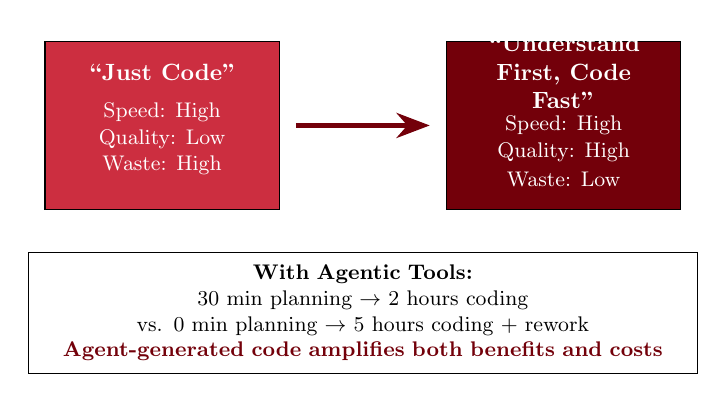
\begin{tikzpicture}[scale=0.85, transform shape]
        % Old mindset
        \node[box=UofSCRose, minimum width=3.5cm, minimum height=2.5cm] (old) at (-4,0) {};
        \node[text=UofSCWhite, font=\bfseries] at (-4,0.8) {``Just Code''};
        \node[text=UofSCWhite, font=\small] at (-4,0.2) {Speed: High};
        \node[text=UofSCWhite, font=\small] at (-4,-0.2) {Quality: Low};
        \node[text=UofSCWhite, font=\small] at (-4,-0.6) {Waste: High};

        % Arrow
        \draw[bigarrow, line width=2pt] (-2,0) -- (0,0);

        % New mindset
        \node[box=UofSCGarnet, minimum width=3.5cm, minimum height=2.5cm] (new) at (2,0) {};
        \node[text=UofSCWhite, font=\bfseries, text width=3cm, align=center] at (2,0.8) {``Understand First, Code Fast''};
        \node[text=UofSCWhite, font=\small] at (2,0) {Speed: High};
        \node[text=UofSCWhite, font=\small] at (2,-0.4) {Quality: High};
        \node[text=UofSCWhite, font=\small] at (2,-0.8) {Waste: Low};

        % Bottom box
        \node[lightbox, minimum width=10cm, minimum height=1.8cm, text width=9.5cm] at (-1,-2.8) {
            \textbf{With Agentic Tools:}\\
            30 min planning $\rightarrow$ 2 hours coding\\
            vs. 0 min planning $\rightarrow$ 5 hours coding + rework\\
            \textcolor{UofSCGarnet}{\textbf{Agent-generated code amplifies both benefits and costs}}
        };
    \end{tikzpicture}
\end{document}
